\section{Optický můstek}
\label{chap:mustek-kap2}
V MO experimentech, ve kterých se měří stočení hlavní roviny polarizace či elipticita, se často využívá schéma optického můstku\footnote{angl. \emph{optical bridge}, také \emph{differential intensity measurement}.}\cite{silberQuadraticMagnetoopticKerr2019a}.
V jednoduché formě je znázorněn na obr. \ref{fig:mustek-schema}.

\begin{figure}[htbp]
    \centering
    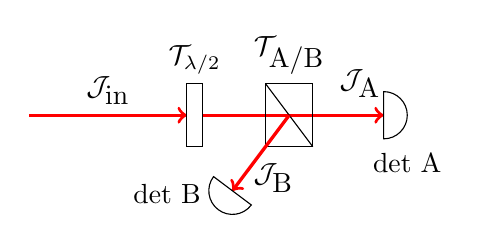
\begin{tikzpicture}[lase/.style={color=red, very thick}]
    \draw[->,lase] (-5,0) -- node[anchor=south,color=black] {$\mathcal{J}_\textrm{in}$} (-3,0);
    \draw (-3,-0.4) rectangle (-2.8,0.4);
    \path (-2.9,0.4) node[anchor=south] {$\mathcal{T}_{\lambda/2}$};
    \draw[->,lase] (-2.8,0) -- (-0.5,0);
    \draw (-2,-0.4) rectangle (-1.4,0.4);
    \draw (-2,0.4) -- (-1.4,-0.4);
    \draw (-0.5,0.3) arc [start angle=90, end angle=-90, radius=0.3cm] -- cycle;
    
    \path (-0.8,0.1) node[anchor=south] {$\mathcal{J}_\textrm{A}$};
    \path (-1.7,0.4) node[anchor=south] {$\mathcal{T}_\textrm{A/B}$};

    \draw[->,lase] (-1.7,0) -- ++(233.1:1.2cm);
    \path +(-1.9,-0.8) node {$\mathcal{J}_\textrm{B}$};
    \draw (-1.7,0) ++(233.1:1.2cm) ++(143.1:0.3cm)  arc [start angle=143.1, end angle=323.1, radius=0.3cm] -- cycle;
    \path (-2.7,-1) node[anchor=east] {det B};
    \path (-0.2,-0.6) node {det A};
\end{tikzpicture}

    \caption{Optický můstek. Naznačeny jsou Jonesovy vektory v určitých místech a matice jednotlivých prvků.}
    \label{fig:mustek-schema}
\end{figure}

Ústředním prvkem je polarizační dělič (často typu Glan Laser či Wollastonův hranol), který rozdělí svazek do dvou lineárně polarizovaných ramen.
Při měření je nejprve nastaven úhel rotace půlvlnné destičky $\theta_{\lambda/2}$ (tzv. ``vyvážení můstku'') tak, aby oba detektory naměřily stejnou intenzitu.
Pro ideální prvky platí v Jonesově formalismu
\begin{align}
    \J_\textrm{A} = \mathcal{T}_\textrm{A} \mathcal{T}_{\lambda/2} \J_\textrm{in} \,&, \quad 
    \mathcal{T}_\textrm{A}=\begin{pmatrix} 0&0\\0&1 \end{pmatrix} \,, \\
    \J_\textrm{B} = \mathcal{T}_\textrm{B} \mathcal{T}_{\lambda/2} \J_\textrm{in} \,&, \quad
    \mathcal{T}_\textrm{B}=\begin{pmatrix} 1&0\\0&0 \end{pmatrix} \,,\\
    \mathcal{T}_{\lambda/2}=\mathcal{R}(\theta_{\lambda/2})\begin{pmatrix} 1&0\\0&-1 \end{pmatrix}\mathcal{R}(-\theta_{\lambda/2}) \,&, \quad
    \mathcal{R}(\theta)=\begin{pmatrix} \cos\theta&-\sin\theta\\\sin\theta&\cos\theta \end{pmatrix} \,.
\end{align}

Dosazením Jonesova vektoru \eqref{eqn:Jones-elipsa} pro natočení hlavní roviny polarizace $\beta$ a elipticitu $\chi$ dostaneme rozdíl intenzit
\begin{equation}
    I_\textrm{A}-I_\textrm{B}\equiv\J_\textrm{A}^\dagger\J_\textrm{A}-\J_\textrm{B}^\dagger\J_\textrm{B}=-I\cos2\chi \cos(2\beta-4\theta_{\lambda/2}) \,, \quad I_\textrm{A}+I_\textrm{B}=I
\end{equation}

Vyvážením můstku nastavíme $\cos(2\beta-4\theta_{\lambda/2})=0$. 
V řeči diferenciálních forem pak pro malé změny $\J_\textrm{in}$ (vyjádřené pomocí $\textrm{d}\beta, \textrm{d}\chi, \textrm{d}I$) platí
\begin{equation}
\label{eqn:A-B-mustek}
    \textrm{d}(I_\textrm{A}-I_\textrm{B})=\pm 2I\cos(2\chi) \textrm{d}\beta \,,
\end{equation}
kde znaménko je určeno tím, jaký konkrétní uzel $\cos(2\beta-4\theta_{\lambda/2})$ byl vyvážením můstku nastaven.
V měřeném signálu se tedy neprojeví změny elipticity ani intenzity.
Pro vstupní lineární polarizaci ($\chi=0$) můžeme měřený rozdílový signál normovat součtovým a dostat
\begin{equation}
\label{eqn:mustek-delta-beta}
    \frac{1}{2}\frac{I_\textrm{A}-I_\textrm{B}}{I_\textrm{A}+I_\textrm{B}}=\Delta\beta \,,
\end{equation}
kde jsme označili $\Delta\beta$ stočení polarizace.
Vhodným vložením čtvrtvlnné destičky lze měřit i elipticitu\cite{silberQuadraticMagnetoopticKerr2019a}.

Optický můstek vždy měří pouze relativní změny $\Delta\beta$ (příp. $\Delta\chi$) vůči vyváženému stavu, který se nemusí shodovat s ``referenčním''\footnote{Většinou nedosažitelný stav $\vec{M}=0$.} stavem, vůči kterému je $\Delta\beta$ modelováno.
Tuto skutečnost vyjadřujeme neznámou aditivní konstantou $\xi$ ($\Delta\beta_\textrm{měření}=\Delta\beta_\textrm{model}+\xi$).

Optický můstek zlepšuje úroveň šumu dvěma způsoby.
Zaprvé se neprojevují fluktuace intenzity (jsou stejné v obou ramenech); zadruhé pak dochází k odečítání blízkých signálů již na úrovni předzesilovače.
Detailnějšímu popisu optického můstku se věnuje oddíl \ref{chap:detekce}.

